\section{Πειραματική Αξιολόγηση}
\subsection{Ερώτημα i}
Ζητείται να εκτελέσουμε όλα τα benchmarks για κάθε διαφορετικό επεξεργαστή που
προκύπτει από το συνδυασμό των παρακάτω τιμών για τις παραμέτρους dispatch\_width
και window\_size:

\begin{center}
   \vspace{3mm}
   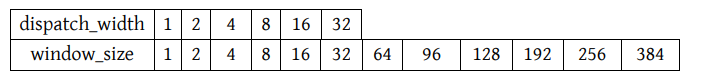
\includegraphics[width=0.9\textwidth]{./imgs/combos.png}
   \vspace{3mm}
\end{center}

\noindent Από τους παραπάνω $6 \times 12  = 72$ δυνατούς συνδυασμούς νόημα έχουν
μόνο εκείνοι για τους οποίους ισχύει $window\_size \geq dispatch\_width$. Αυτό
μπορεί να γίνει αντιληπτό θεωρητικά αν μελετήσουμε τον τρόπο με τον οποίο
γίνονται dispatch για issue οι εντολές και το ρόλο του Reorder Buffer (ROB) Όπως
γνωρίζουμε για να γίνει μία εντολή issue πρέπει να υπάρχει διαθέσιμη θέση στον
ROB. Επομένως, είναι χωρίς νόημα να κάνουμε dispatch παραπάνω εντολές από όσες
μπορούν να χωρέσουν στον Reorder Buffer, γιατί απλά αυτές θα περιμένουν μέχρι να
υπάρξει ελεύθερη θέση στον ROB και άρα η επίδοση δε θα βελτιωθεί καθόλου. Με
βάση αυτό αγνοούμε για οικονομία χρόνου στις προσομοιώσεις τους συνδυασμούς για
τους οποίους $window\_size < dispatch\_width$ και εκτελούμε τους εναπομείναντες
57 διαφορετικούς συνδυασμούς. 

Την παρατήρηση αυτή μπορούμε να επιβεβαιώσουμε και περιματικά. Στα παρακάτω
διαγράμματα απεικονίζεται η μετρική Instructions Per Cycle για τα
μετροπρογράμματα gcc και sjeng για όλους τους δυνατούς συνδυασμούς. Παρατηρούμε
πως για κάθεμία από τις καμπύλες των διαγραμμάτων (που ανατιστοιχεί σε ορισμένο
dispatch width), η απόδοση (IPC) για τις τιμές windows\_size που είναι μκρότερες από 
το dispatch width είναι αρκετά χαμηλή.

\vspace{3mm}
   \begin{minipage}{\textwidth}
      \begin{center}
         \fbox{\textlatin{\textbf{\textit{403-gcc}}}}\\
         \vspace{3mm}
         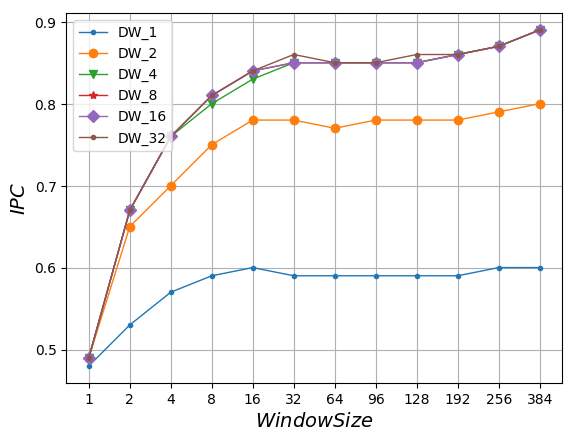
\includegraphics[width=0.7\textwidth, frame]{./graphs/ipc/gcc.png}
         \vspace{6mm}
      \end{center}
   \end{minipage}

   \begin{minipage}{\textwidth}
      \begin{center}
         \fbox{\textlatin{\textbf{\textit{458-sjeng}}}}\\
         \vspace{3mm}
         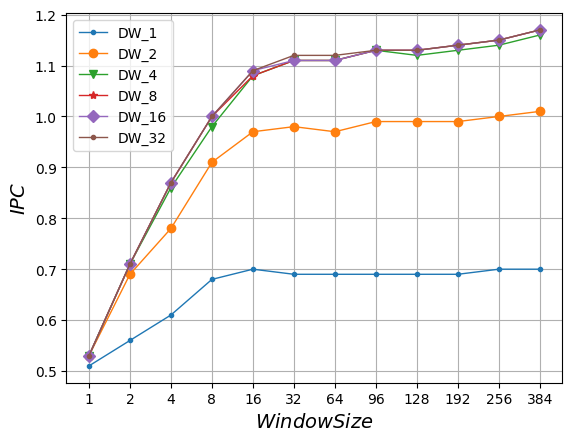
\includegraphics[width=0.7\textwidth, frame]{./graphs/ipc/sjeng.png}
         \vspace{6mm}
      \end{center}
   \end{minipage}
